\documentclass[final]{beamer}
\usepackage[orientation=portrait,size=a1,scale=1.25]{beamerposter}
\usetheme[facepic=]{JDOC}

\usepackage[utf8]{inputenc}
\usepackage[frenchb]{babel}
%\usepackage{lmodern} 
\usepackage{subcaption}

% TODO:
% - advisors' names
% - picture

\title{\Huge{\textbf{Génération de Modèles pour l'Analyse Temporelle}}}
\author{Armel Mangean \\
  \texttt{armel.mangean@irccyn.ec-nantes.fr}}

\institute{%
  Spécialité : Informatique \\
  Laboratoire : IRCCyN \\
  Équipe : Sytèmes Temps-Réel \\
  Directeur : Jean-Luc Béchennec \\
  Encadrant : Sébastien Faucou}

\begin{document}
  \begin{frame}
  
    \begin{columns}[t]
      \begin{column}{.45\linewidth}
        %%% Problèmatique
        \section{Estimer un pire cas de temps d'exécution ? \\
          {\small ou \emph{Worst Case Execution Time} (WCET)}}
        \begin{figure}[ht]
          \centering
          \captionsetup{justification=centering}
          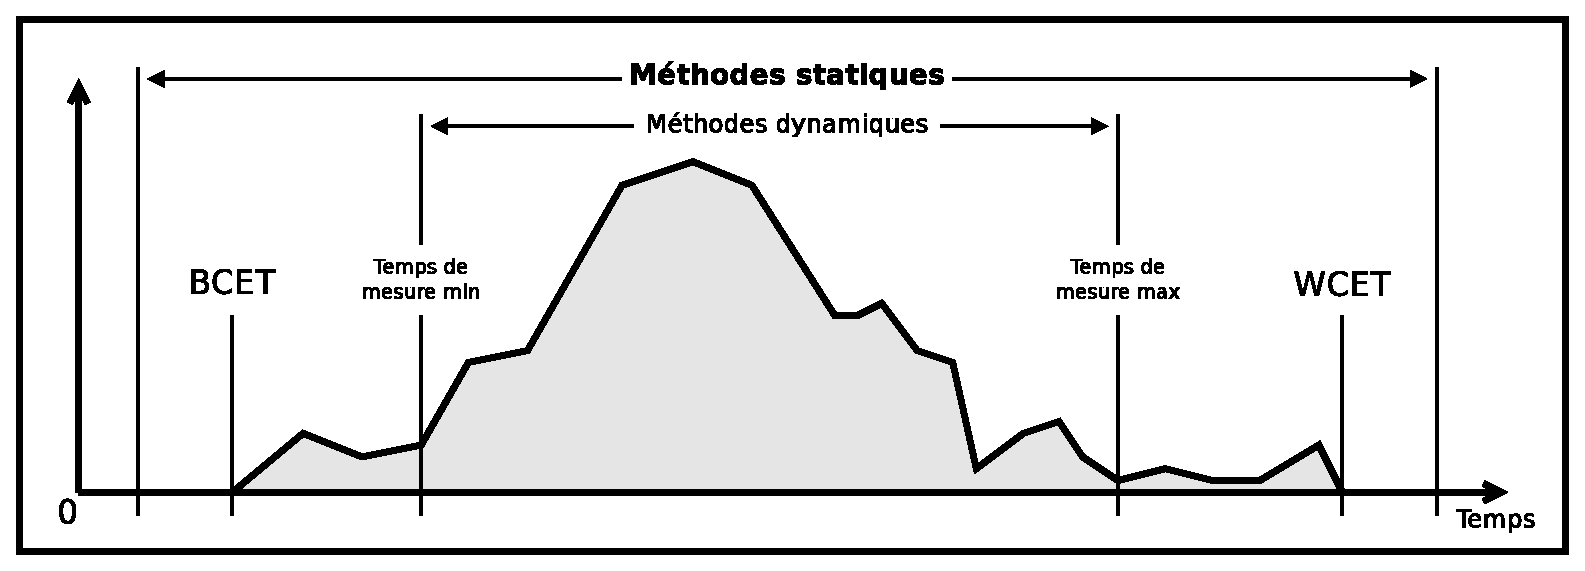
\includegraphics[scale=.8]{img/wcet.eps}
          \caption{Distribution de temps d'exécutions}
          \label{fig:wcet}
        \end{figure}
        \vspace{1em}
        \begin{block}{Différentes méthodes d'estimation}
          \begin{itemize}
            \item Méthodes dynamiques
              \begin{itemize}
                \item[$\Rightarrow$] Jeux de tests et mesures
                \item Sous-approximations du pire cas \\
                  $\rightarrow$ pas sûr
              \end{itemize}
            \vspace{.5em}
            \item \textbf{Méthodes statiques}
              \begin{itemize}
                \item[$\Rightarrow$] Interprétation abstraite, \textbf{vérification de modèles}
                \item Sur-approximations du pire cas \\
                  $\rightarrow$ sûr mais souvent peu précis
              \end{itemize}
          \end{itemize}
        \end{block}
      \end{column}
      
      \begin{column}{.45\linewidth}
        %%% Notre approche
        \section{Estimation de WCET \\
          par vérification de modèles \\
          {\small ou Analyse temporelle par \emph{model checking}}}
        \begin{figure}
          \centering
          \captionsetup{justification=centering}
          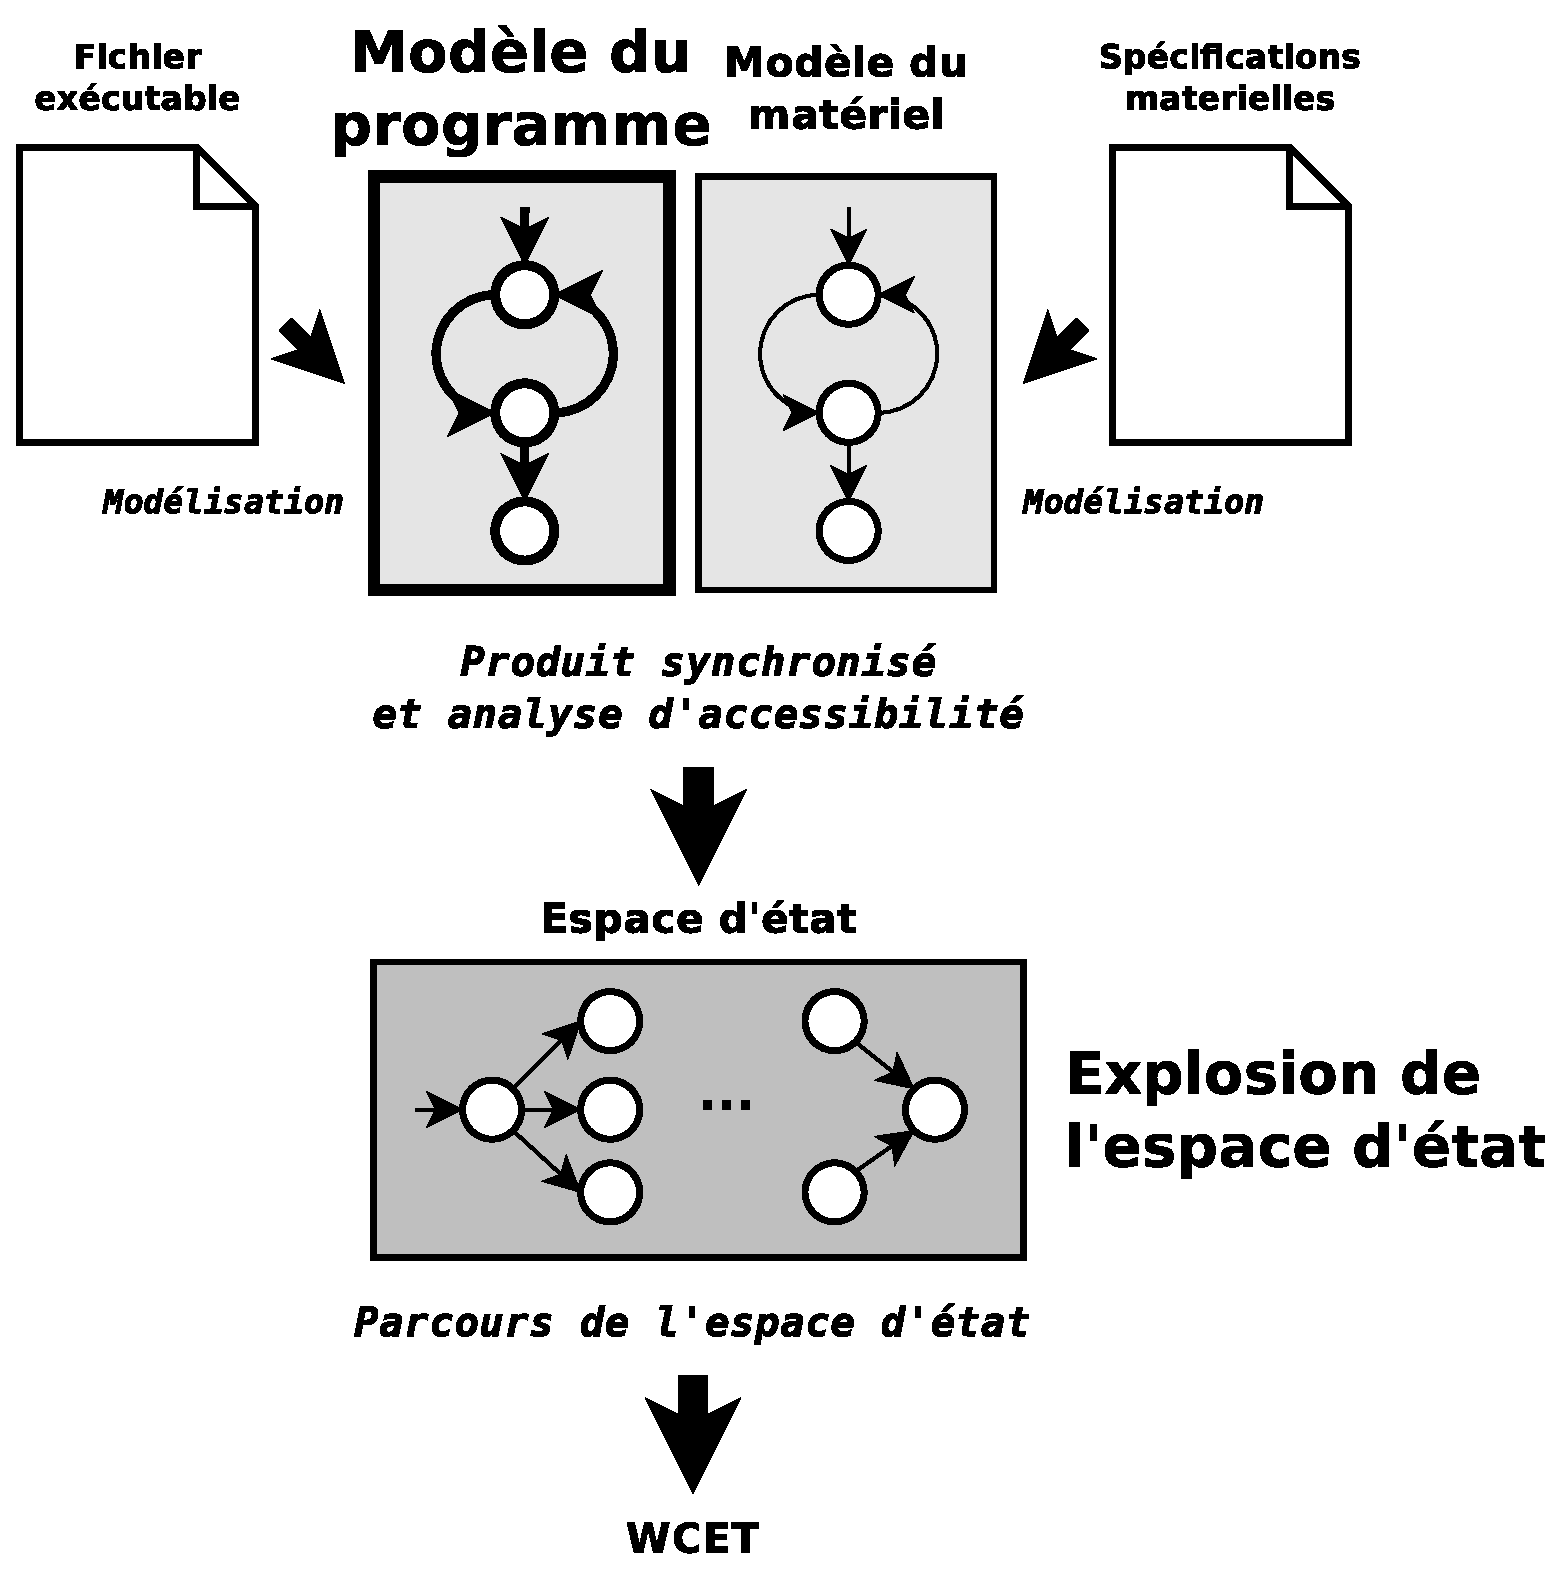
\includegraphics[scale=.66]{img/model-checking.eps}
          \caption{Principes de l'analyse temporelle \\
            ~~~~ par \emph{model checking}}
          \label{fig:analyse}
        \end{figure}
      \end{column}
    \end{columns}

    %%% Mise en oeuvre (théorique)
    \section{Génération de modèles de programme}
    \begin{columns}[t]      
      \begin{column}{.66\linewidth}
        \begin{figure}[ht]
          \centering
          \begin{subfigure}{.30\textwidth}
            \centering
            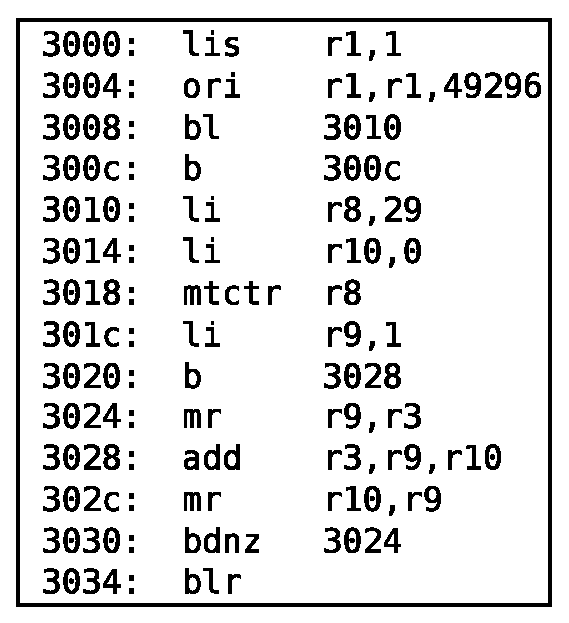
\includegraphics{img/dump-new.eps}
            \captionsetup{justification=centering}
            \caption{\emph{Dump} du programme \\
              (désassemblage du fichier exécutable)}
            \label{fig:dump}
          \end{subfigure}
          \begin{subfigure}{.30\textwidth}
            \centering
            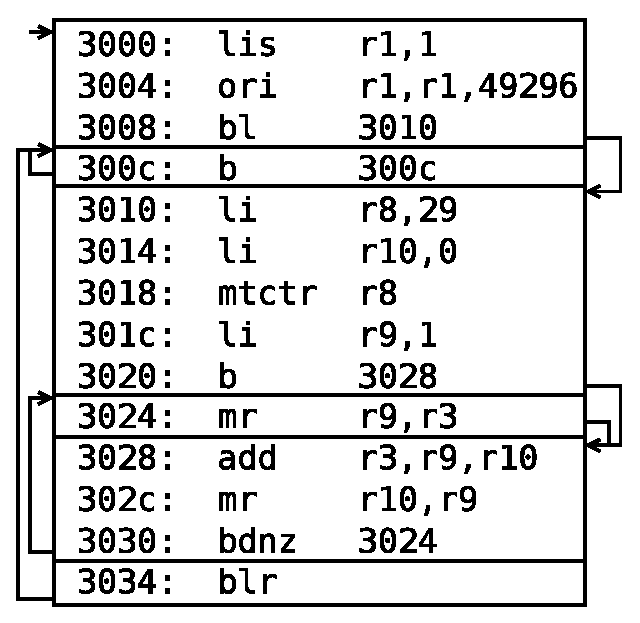
\includegraphics{img/recons-new.eps}
            \captionsetup{justification=centering}
            \caption{Graphe de flot de contrôle \\
              \textbf{\emph{Control Flow Graph} (CFG)}}
            \label{fig:recons}
          \end{subfigure}
          \begin{subfigure}{.30\textwidth}
            \centering
            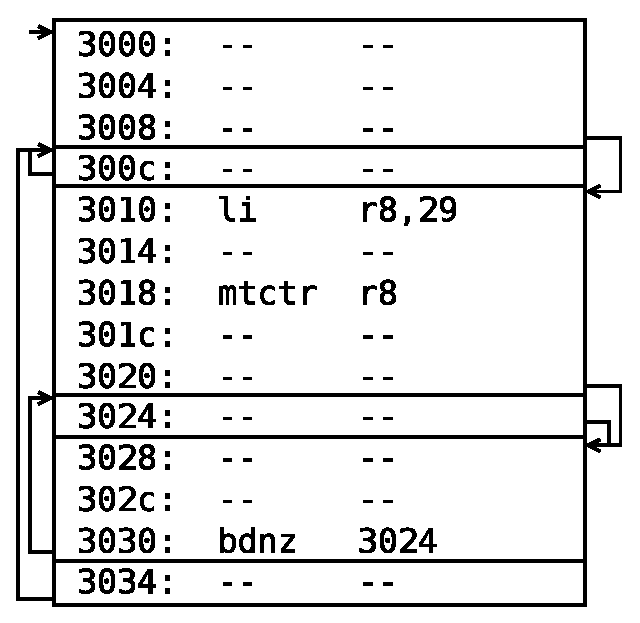
\includegraphics{img/slice-new2.eps}
            \captionsetup{justification=centering}
            \caption{\textbf{\emph{slice} du CFG} pour le critère \\
              $\mathcal{C} = \langle 3030, \{ ctr \} \rangle$}
            \label{fig:slice2}
          \end{subfigure}
          \caption{Génération du modèle du programme << \texttt{fibcall-O2.elf} >>}
        \end{figure}
      \end{column}
      \begin{column}{.33\linewidth}
        \begin{block}{Approche et intérts}
          \begin{itemize}
            \item Approche
              \begin{itemize}
                \item Reconstruction du CFG
                \item \emph{Program slicing} du CFG {\color{jdocgreen1}[4]}
                \item Construction d'un automate fini
              \end{itemize}
              \vspace{.5em}
          
              \item Intérêts
                \begin{itemize}
                  \item Utilisation d'un modèle exact du programme
                  \item Réduction de l'espace d'état engendré \\
                    \begin{center}
                      $\rightarrow$ Permet l'utilisation d'un modèle exact du materiel pour réaliser l'analyse temporelle \\
                      \vspace{.5em}
                      $\Rightarrow$ \textbf{Approximation précise du WCET}
                    \end{center}
                \end{itemize}
          \end{itemize}
        \end{block}
      \end{column}
    \end{columns}
    
    %%% Mise en oeuvre (théorique)
    \section{Implémentation}

    \begin{columns}[t]
      \begin{column}{.66\linewidth}
        \begin{figure}
          \centering
          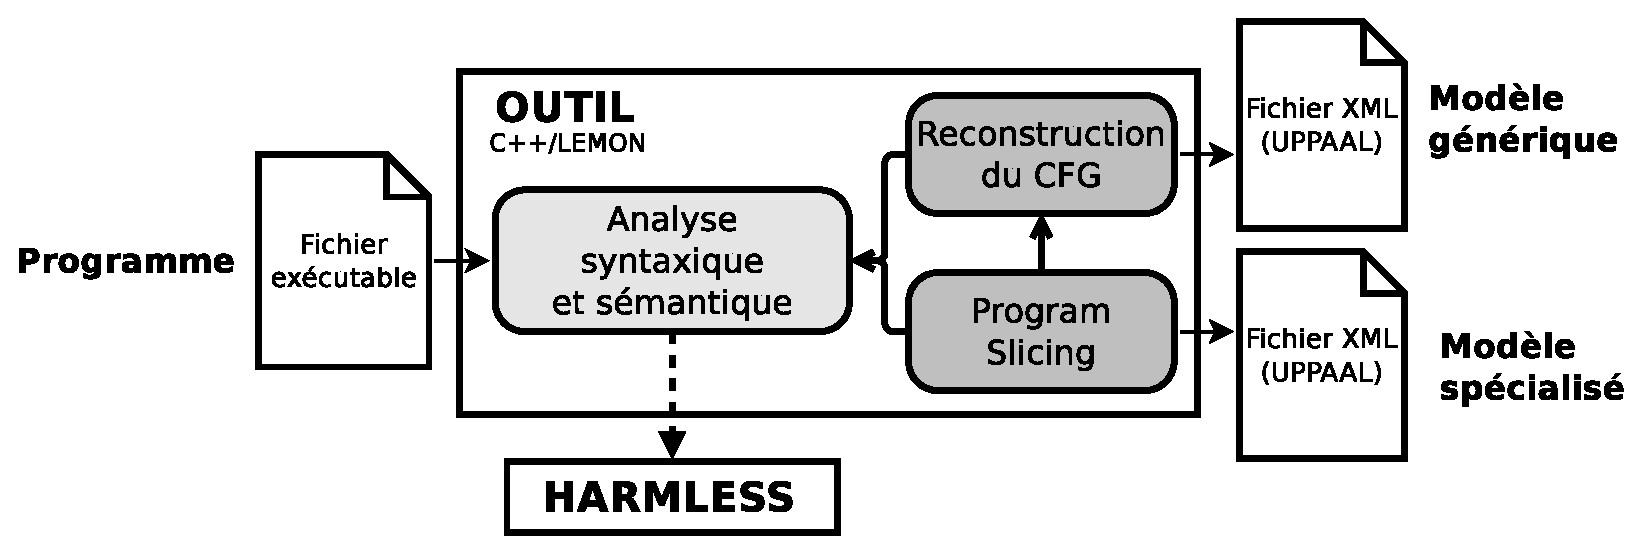
\includegraphics{img/archi.eps}
          \caption{Implémentation}
          \label{fig:tool}
        \end{figure}
      \end{column}
      \begin{column}{.33\linewidth}
        \begin{block}{Détails}
          \begin{description}[HARMLESS]
            \item[HARMLESS] Générateur de simulateurs d'architectures d'ordinateurs {\color{jdocgreen1}[3]}
            \item[LEMON] Bibliothèque de manipulation de graphes {\color{jdocgreen1}[2]}
            \item[UPPAAL] \emph{Model checker} temporisé
          \end{description}
        \end{block}
      \end{column}
    \end{columns}

    
    
    % Conclusion et perspectives
    %\section{Conclusion et perspectives}
      \subsection{Références}
      %% \nocite{*}
      %% \bibliographystyle{plain}
      %% \bibliography{refs}
      
      \small
      
      {\color{jdocgreen1} [1]} Franck Cassez and Jean-Luc Bechennec. Timing Analysis of
      Binary Programs with UPPAAL. In 2013 13th International Conference on Application of
      Concurrency to System Design (ACSD), pages 41–50. IEEE, 2013. {\color{jdocgreen1}
        [2]} Balázs Dezső, Alpár Jüttner, and Péter Kovács. LEMON – an Open Source C++
      Graph Template Library. Electronic Notes in Theoretical Computer Science, 264(5)
      :23–45, 2011. {\color{jdocgreen1} [3]} Rola Kassem, Mikaël Briday, Jean-Luc
      Béchennec, Guillaume Savaton, and Yvon Trinquet. Harmless, a hardware architecture
      description language dedicated to real-time embedded system simulation. Journal of
      Systems Architecture, 58(8) :318–337, September 2012. {\color{jdocgreen1} [4]} Akos
      Kiss, Judit Jász, Gábor Lehotai, and Tibor Gyimóthy.  Interprocedural Static Slicing
      of Binary Executables. In Source Code Analysis and Manipulation,
      2003. Proceedings. Third IEEE International Workshop on, pages 118–127. IEEE, 2003.
      
  \end{frame}
\end{document}

